%************************************************
\chapter{Introduction to Learning-to-Rank}
Different definitions of Learning-to-Rank exist. In general, all methods that use machine learning technologies to solve the problem of ranking are called Learning-to-Rank methods.\\
Liu \cite{Liu2007} proposes a more narrow definition and only considers ranking methods to be a Learning-to-Rank method when it meets the following two properties:
\begin{description}
\item[Feature Based]{\emph{Feature based} means that all documents under investigation are represented by feature vectors that reflect the relevance of the documents to the query.}
\item[Discriminative Training]{\emph{Discriminative training} means that the learning process can be well described by the four components of discriminative learning, that is, a Learning-to-Rank method has its own input space, output space, hypothesis space, and loss function. Input space, output space, hypothesis space, and loss function are hereby defined as follows:
	\begin{description}
	\item[Input Space]{contains the objects under investigation. Usually objects are represented by feature vectors, extracted according to different applications.}
	\item[Output Space]{contains the learning target with respect to the input objects.}
	\item[Hypothesis Space]{defines the class of functions mapping the input space to the output space. The functions operate on the feature vectors of the input object, and make predictions according to the format of the output space.}
	\item[Loss Function]{In order to learn the optimal hypothesis, a training set is usually used, which contains a number of objects and their ground truth labels, sampled from the product of the input and output spaces.}
	\end{description}
	}
\end{description}
\begin{figure}[!h]
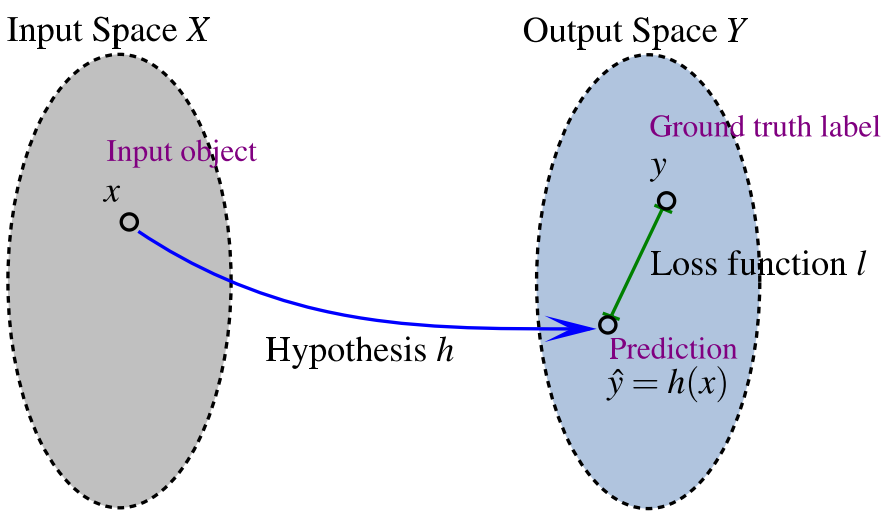
\includegraphics[scale=0.26]{gfx/descriminative_training}
\caption{Machine learning framework for Learning-to-Rank, from Liu\cite{Liu2007}}
\label{fig:discriminative_training}
\end{figure}
Figure \ref{fig:discriminative_training} shows the relationships between input space, output space, hypothesis space and loss function.

Figure \ref{ref:ltr_framework} shows how the learning process in Learning-to-Rank typically happens. A set of queries $q_i$ with $n > i > 1$, the documents associated with these queries which are represented by feature vector $x_i$, and the relevant judgments of those documents $y_i$ are inputted to a learning algorithm that learns a ranking model such that the output of the ranking model can predict relevant judgment labels in this training set as accurately as possible. Later on we can test the accuracy of this ranking model by predicting the relevant judgments new documents given a new query.
\begin{figure}[!h]
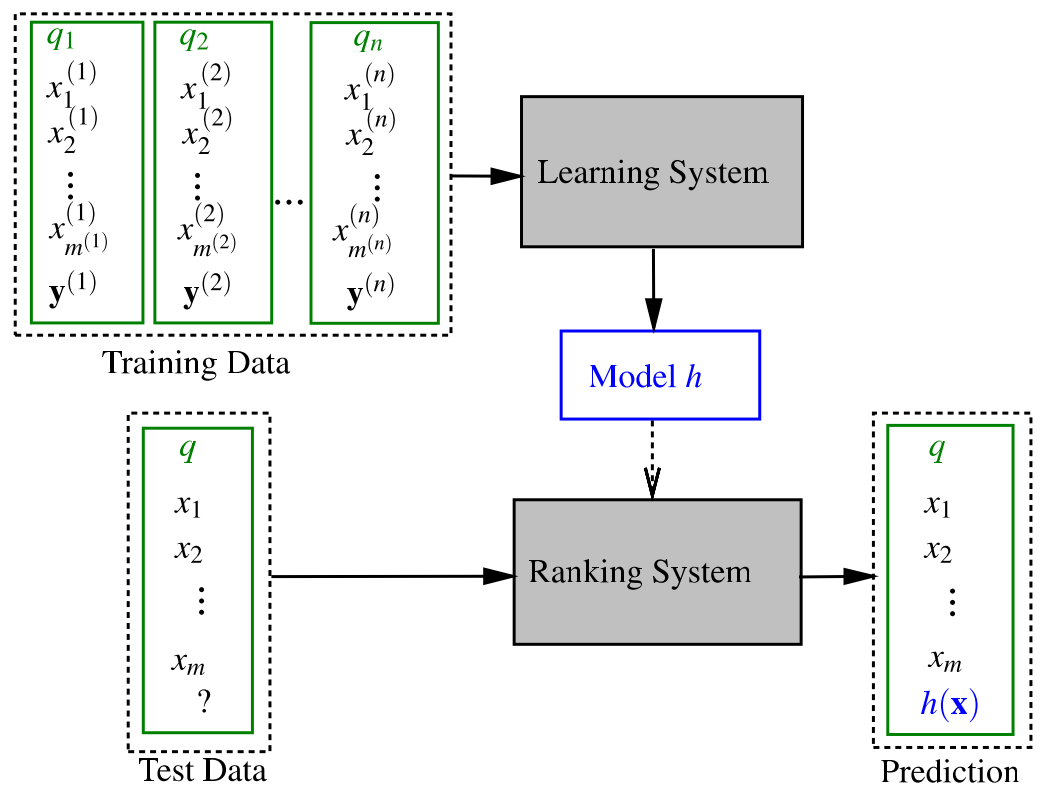
\includegraphics[scale=0.25]{gfx/ltr_framework}
\caption{A typical Learning-to-Rank setting, from Liu\cite{Liu2007}}
\label{ref:ltr_framework}
\end{figure}\\

Learning-to-Rank algorithms can be classified into three approaches: the pointwise approach, the pairwise approach and the listwise approach, on which we will elaborate in the subsequent chapters.

\chapter{Pointwise Approach}
\chapter{Pairwise Approach}
\chapter{Listwise Approach}
\chapter{Summary}